%!TEX root = skripsi.tex
%-----------------------------------------------------------------------------%
\chapter{\babDua}
%-----------------------------------------------------------------------------%
Bab ini membahas mengenai studi literatur yang digunakan selama penelitian. Studi literatur ini menjelaskan tentang hal-hal mendasar yang dibutuhkan dalam penelitian.

%-----------------------------------------------------------------------------%
\section{Word Sense Disambiguation}
%-----------------------------------------------------------------------------%
\textit{Word Sense Disambiguation} merupakan salah satu penelitian di bidang NLP yang bertujuan untuk menentukan makna yang paling tepat dari suatu kata berdasarkan konteks kata tersebut ditemukan. Sebagaimana kata dalam suatu bahasa bisa memiliki makna lebih dari satu (polisemi), \textit{task} ini akan menentukan makna kata mana yang paling tepat. 

Penentuan makna kalimat dilakukan dengan pemberian informasi berupa kata yang menjadi \textit{target} dan konteks berupa kalimat. Contoh proses disambiguasi yang dilakukan untuk kata \textbf{cokelat}:



K1: Roni memakan \textbf{cokelat} yang diberikan ibunya.


K2: Walaupun mobil \textbf{cokelat} itu mahal, dia sangat ingin membelinya.



Pada kalimat pertama (K1), \textbf{cokelat} yang dimaksud memiliki makna sebagai makanan yang terbuat dari buah \textit{cokelat}. Sementara itu, Kata \textbf{cokelat} pada kalimat kedua (K2) memiliki makna yang berbeda, dimana kata tersebut merupakan satu keterangan warna. Penentuan makna yang tepat dapat dilakukan dengan bantuan informasi konteks dari kalimat dimana kata tersebut muncul. Pada K1, kata \textbf{memakan} memberikan informasi bahwa \textit{cokelat} yang dimaksud adalah objek yang bisa dimakan. Kata yang memberikan informasi pada kalimat kedua adalah kata \textbf{berwarna} yang secara eksplisit menerangkan bahwa \textbf{cokelat} yang dimaksud adalah warna. Namun demikian, konteks maupun informasi yang bisa diambil dari kalimat tidak selalu eksplisit. Pada contoh kalimat seperti "Pohon cokelat tua di belakang rumahku sangat besar", cokelat yang dimaksud bisa bermakna "buah cokelat yang sudah tua" atau "berwarna cokelat tua".

Penentuan makna kata yang tepat oleh sistem WSD ditentukan berdasarkan konteks dari kata tersebut berada. Walaupun satu kata dapat memiliki beberapa makna, terdapat kecil kemungkinan bahwa kata yang sama digunakan dalam satu \textit{discourse} untuk menyatakan makna yang berbeda sebagaimana "\textit{one sense per discourse}" \citep{gale1992one}.

\subsection{WSD Bahasa Inggris}
Salah satu sistem WSD untuk bahasa inggris yang ada adalah "It Makes Sense" (IMS) yang dibuat oleh Zhi Zhong dan Hwee Tou Ng \citep{zhong2010makes}. Sistem  dibangun menggunakan pendekatan \textit{supervised learning} yang dapat digunakan untuk semua kata bahasa Inggris. Pada dasarnya, \textit{classifier} yang dipilih untuk \textit{task} ini adalah \textit{support vector machine} (SVM). Arsitektur yang dibangun pada IMS dapat dilihat pada gambar berikut:

\begin{figure}
	\centering
	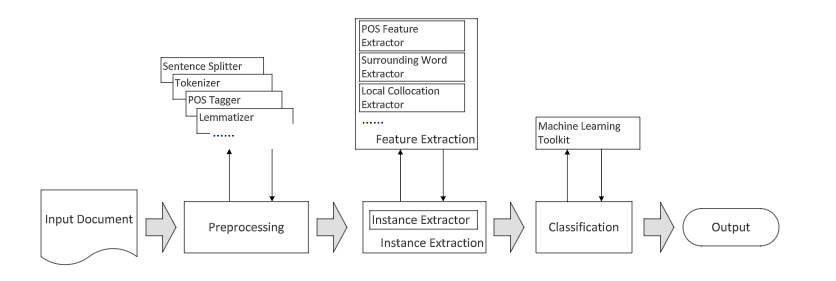
\includegraphics[width=1\linewidth]{adit_pics/Arsitektur-IMS}
	\caption{Arsitektur IMS}
	\label{fig:Arsitektur-IMS}
\end{figure}

Proses \textit{pre-processing} pada IMS dilakukan dengan empat tahapan:
\begin{enumerate}
	\item Mendeteksi batasan kalimat dengan \textit{sentence splitter}
	\item Tokenisasi dengan \textit{tokenizer}
	\item POS Tagging untuk semua token
	\item Mengubah token menjadi lemma dengan \textit{lemmatizer}
\end{enumerate}

Ekstraksi fitur dilakukan dengan mengombinasikan:

\begin{enumerate}
	\item POS Tag dari tiga buah kata di kiri dan kanan \textit{target word}, serta kata itu sendiri. 
	\item Kata-kata sekitar pada konteks kalimat ataupun kalimat tetangganya. Kata-kata yang terkandung di dalam \textit{stopwords} dan memiliki simbol atau angka dibuang dari kalimat tersebut. Kata-kata yang tersisa tersebut kemudian diubah menjadi bentuk kata dasarnya dalam huruf kecil.
	\item \textit{Local Collocation} dengan 11 buah \textit{collocation} baik itu sebelum \textit{target word} maupun setelahnya. 
\end{enumerate}

Pengujian seberapa baik performa IMS dalam melakukan  WSD \textit{task} mendapatkan hasil:

\begin{figure}
	\centering
	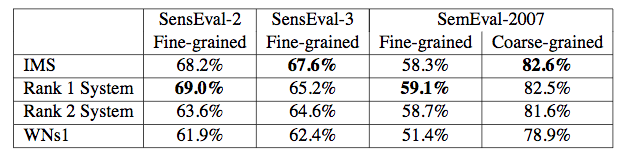
\includegraphics[width=1\linewidth]{adit_pics/Performa-IMS}
	\caption{Performa IMS \citep{zhong2010makes}}
	\label{fig:Performa-IMS}
\end{figure}

\subsection{WSD \textit{Cross Language}}

Salah satu penelitian yang ada terkait dengan \textit{cross language} WSD dilakukan untuk antara bahasa Quechua dan Spanyol \citep{rudnick2011towards}. Penelitian tersebut dilakukan untuk menghasilkan sebuah sistem WSD yang nantinya dapat diintegrasikan dengan \textit{Machine Translation System} untuk bahasa tersebut. Kata yang menjadi fokus pada penelitian tersebut hanyalah \textit{adjective word} saja, karena sedikitnya kata infleksional dalam bahasa Quechua. Terdapat dua buah kamus digital yang digunakan untuk melakukan penerjemahan kata antara kedua bahasa. Wordnet bahasa Spanyol yang digunakan bukan sepenuhnya Wordnet \textit{full version} yang membutuhkan biaya dan \textit{lisence} untuk dapat diakses, namun merupakan subset dari Wordnet \textit{full version} tersebut. Korpus yang digunakan sebagai \textit{paralel resource text} merupakan Bitext (bibel Katolik) dengan total 31 ribu jumlah ayat.

Proses ekstraksi kata-kata yang ambigu dari kamus kedua bahasa dilakukan dengan cara menetapkan kata-kata dalam bahasa Spanyol yang dapat diterjemahkan menjadi lebih dari satu kata dalam bahasa Quechua yang berbeda (dengan tipe kelas kata adalah \textit{adjective}).

Setelah mendapatkan kata-kata ambigu pada bahasa Spanyol tersebut, proses berikutnya adalah mencari dan mengumpulkan ayat yang mengandung kata ambigu tersebut untuk data \textit{training}.

Proses disambiguasi yang dicoba menggunakan beberapa cara diantaranya KNN yang memperhitungkan jarak terdekat kedua node kata pada Wordnet, Simplified lesk Algorithm, dan penggunakan fitur untuk \textit{classifier} tertentu. Pendekatan fitur yang digunakan adalah kata samping dari \textit{target word}, synsets dari Wordnet Spanyol untuk kata tetangganya, dan hasil \textit{parse} dengan menggunakan \textit{dependancy parser}. Semua fitur tersebut dicoba pada \textit{classifier} KNN, decision tree, dan naive bayes.


\begin{figure}
	\centering
	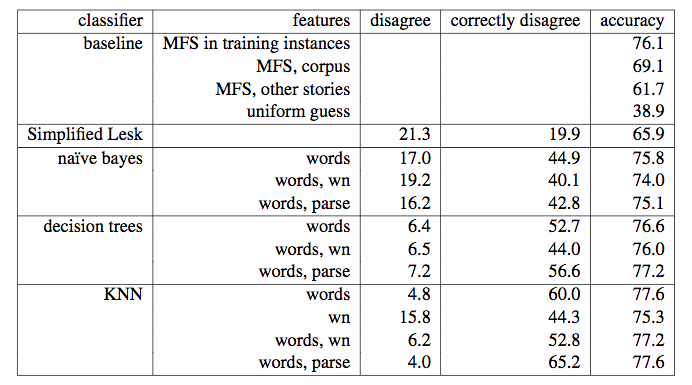
\includegraphics[width=1\linewidth]{adit_pics/crosslanguage-wsd}
	\caption{Akurasi Klasifikasi dari penelitian \citep{rudnick2011towards} dengan cross validation}
	\label{fig:akurasi-klasifikasi}
\end{figure}

Simplified Lesk dalam percobaan tersebut menghadapi kasus dimana tidak terdapat kata yang ditemukan dari konteks word pada entri kamus. Fitur yang menghasilkan akurasi terbaik dari percobaan tersebut merupakan KNN dengan fitur konteks kata dengan fitur \textit{parser}.

%-----------------------------------------------------------------------------%
\section{Word Sense Induction}
%-----------------------------------------------------------------------------%	
%-----------------------------------------------------------------------------%	
\textit{Word Sense Induction} (WSI) adalah sebuah \textit{task} yang mempunyai fungsi utama untuk mendapatkan makna kata dari sebuah korpus atau teks yang belum dianotasi secara otomatis. WSI dapat dilakukan jika penelitian WSD yang ingin dilakukan tidak mempunyai cukup \textit{resource} seperti misalnya Wordnet yang memadai. Terdapat berbagai macam pendekatan dalam melakukan WSI, diantaranya adalah dengan melakukan \textit{clustering} kata \citep{denkowski2009survey}, ataupun menggunakan pendekatan \textit{cross language}.
	
	\subsection{Pendekatan \textit{Clustering}}
	Dua kata dianggap dekat secara semantik jika memiliki \textit{co-occurrence} dengan kata-kata tetangganya yang sama \citep{nasiruddin2013state}. Konsep tersebut mendasari cara WSI mendapatkan \textit{sense} kata secara implisit berdasarkan hasil \textit{cluster} yang terbentuk dari data atau teks mentah (teks yang tidak dianotasi).
	
	Penarikan makna secara implisit dapat dicontohkan pada beberapa kalimat rujukan berikut \citep{denkowski2009survey}:
	
	\begin{enumerate}
		\item A bottle of tezg\"{u}no is on the table.
		\item Everyone likes tezg\"{u}no.
		\item Tezg\"{u}no makes you drunk.
		\item We make tezg\"{u}no out of corn.
	\end{enumerate}
	
	Walaupun belum terdapat informasi eksplisit makna dari tezg\"{u}no, dapat disimpulkan bahwa tezg\"{u}no mengacu pada minuman beralkohol yang memabukkan. Penarikan kesimpulan ini didapatkan dari kemunculan kata tersebut dengan kata lain pada konteks yang sama.
	
	Pada pendekatan \textit{clustering} ini, makna kata bisa didapatkan secara implisit dari hasil \textit{cluster} yang terbentuk, namun demikian pelabelan yang dilakukan untuk menentukan apa yang direpresentasikan \textit{cluster} tersebut merupakan sebuah \textit{task} tersendiri.
	
	\subsection{Pendekatan \textit{Cross Language}}
	Selain pendekatan \textit{clustering}, WSI juga dapat memanfaatkan fitur dimana satu kata dari suatu bahasa, dapat diterjemahkan menjadi beberapa kata di bahasa lain. Contoh kasus tersebut dapat dilihat pada kata "halaman" berikut:



	(K1-Indonesia): Aku membaca 10 \textbf{halaman} buku Harry Potter
	
	(K1-English): I read 10 \textbf{pages} of Harry Potter book
	
	(K2-Indonesia): Ani tinggal di rumah dengan \textbf{halaman} yang sangat luas
	
	(K2-English): Ani lives in a house with very large \textbf{yard}
	
	
	
	Berdasarkan kedua pasangan kalimat tersebut, kata \textbf{halaman} dalam bahasa Indonesia dapat diterjemahkan menjadi dua buah kata dalam bahasa Inggris, yaitu \textit{page} ataupun \textit{yard}. Hal ini menunjukan bahwa terjemahan dari suatu kata bergantung pada konteks dimana kata tersebut muncul.


\section{Korpus Paralel dan \textit{Comparable}}
Terdapat dua macam korpus bilingual yang dapat dimanfaatkan untuk pemanfaatan \textit{cross language } WSD yaitu korpus paralel dan \textit{comparable}. Perbedaan utama terhadap kedua buah korpus berada pada seberapa identik kedua buat kontek yang dimilikinya. Korpus paralel memiliki kalimat dan kata-kata yang serupa antara dua buah pasangan \textit{instance} di masing-masing korpus. Hal ini dapat dicontohkan misalnya dengan kalimat satu pada korpus bahasa Indonesia "Aku makan" dengan "I eat" pada korpus bahasa Inggris. Berbeda dengan korpus paralel, \textit{comparable} berarti kedua kalimat atau \textit{instance} yang berpasangan hanya sebatas mirip/sama dalam suatu kategori kriteria tertentu. Dengan adanya korpus paralel dan \textit{comparable} tersebut, dibutuhkan juga alat untuk menyelaraskan (\textit{aligning}) konten pada kedua korpus tersebut. \textit{Alignment} yang dapat dilakukan memiliki beberapa tingkatan mulai dari \textit{scope} yang besar sampai kecil. \textit{Scope} besar tersebut meliputi \textit{alignment} dokumen yang mana fungsinya adalah menyelaraskan antar dokumen yang konten atau kriterianya sama. Tingkatan yang lebih kecil berikutnya yaitu kalimat dimana \textit{alignment} dilakukan pada \textit{level} kalimat (pasangan kalimat yang makna atau kriterianya sama). \textit{Alignment} dengan tingkatan yang lebih spesifik lagi adalah kata (\textit{word alignment}), dimana hasil yang didapat dari proses ini adalah pasangan kata pada kedua korpus dwibahasa yang selaras.
%-----------------------------------------------------------------------------%
\section{\textit{Word Alignment}}

\subsection{\textit{Task Word Alignment}}
Tugas dari \textit{word alignment} adalah menemukan korespondensi antara kata dan frasa pada teks paralel 
\citep{mihalcea2003evaluation}. Evaluasi ini akan membandingkan antara hasil \textit{alignment} dari sebuah tool \textit{word alignment} dengan hasil \textit{alignment} manusia sebagai \textit{gold standard}. Kasus yang dapat terjadi pada proses \textit{alignment} ini adalah ketika terdapat kata yang tidak memiliki pasangan. Contoh dari kasus tersebut dapat dilihat pada pasangan kaimat berikut:


K1(en) : \textit{He would do it regardless what people say}

K1(id) : Dia akan melakukannya segalanya


Bila melihat bahasa Indonesia sebagai sumber bahasa, maka kata "segalanya" pada kalimat tersebut tidak memiliki pasangan. Pada kasus seperti contoh diatas, kata yang tidak memiliki pasangan akan dipasangkan dengan \textit{token} NULL.


Selain kata yang tidak memiliki pasangan, terdapat juga kasus dimana pasangan adalah berupa frasa. Hal ini dapat dilihat pada contoh berikut:


K2(en) : The victim must be taken to the hospital

K2(id) : Korban tersebut harus di bawa ke rumah sakit


Berangkat dari bahasa asal yaitu Indonesia, kata "rumah sakit" dipasangkan kepada kata "hospital". Hal ini dapat berlaku berkebalikan jika bahasa asal yang digunakan adalah bahasa Inggris seperti kata "untuknya" berpasangan dengan kata "for him".

\subsection{Representasi Kalimat}

Pada penelitian \citep{mihalcea2003evaluation}, pemisah kata yang umum digunakan untuk tokenisasi adalah karakter spasi. setiap token dari hasil tokenisasi tersebut kemudian dianggap sebagai satu unit kata. Kata ini akan diindeks dengan angka untuk mempermudah proses \textit{alignment} dan komputasi evaluasi. Contoh tokenisasi dan pemberian indeks pada kalimat "Aku ingin membeli mainan" adalah:

K3(id) : Aku ingin membeli mainan

K3(indeks) : 1 2 3 4

Angka yang menjadi indeks tersebut akan merepresentasikan kata yang bersesuaian, indeks 1 mewakili kata "Aku", indeks 2 mewakili "ingin", dan lain-lain. Beberapa \textit{tool} merepresentasikan kalimat dan kata sebagai indeks angka tersebut untuk mempermudah pemrosesan tahap-tahap selanjutnya. Suatu \textit{file} dapat berisi indeks dari kalimat dan kata yang ada pada kalimat tersebut seperti:
\begin{lstlisting}
1 4 5 7
2 4 9 2
3 1 8 4
...
\end{lstlisting}

Dimana angka pertama merepresentasikan kalimat ke n pada korpus, dan angka-angka selanjutnya adalah indeks dari kata pada kalimat tersebut.

\subsection{Pengukuran Evaluasi}
Terdapat empat buah pengukuran berbeda, yaitu \textit{precision}, \textit{recall}, \textit{f-measure}, dan \textit{alignment error rate (AER)} \citep{mihalcea2003evaluation}. Diberikan hasil \textit{alignment} dari program berupa A, dan \textit{gold standard alignment} dari \textit{evaluator} (manusia) sebagai G, masing-masing mengandung dua buah \textit{set} yaitu \textit{probable alignment} dan \textit{sure alignment}. Pengukuran evaluasi dapat dilakukan dengan cara berikut:

\begin{figure}
	\centering
	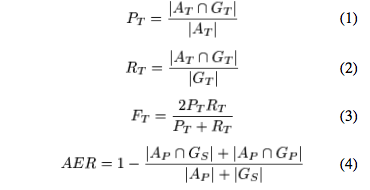
\includegraphics[width=1\linewidth]{adit_pics/Pengukuran-Word-Alignment}
	\caption{Pengukuran Word Alignment}
	\label{fig:Pengukuran-Word-Alignment}
\end{figure}

Dikarenakan proses \textit{word alignment} pada penelitian ini tidak membedakan antara \textit{probable} dan \textit{sure alignment}, maka semua dianggap merupakan set dari \textit{sure alignment}.
%------------------------------------------- ----------------------------------%

\section{Support Vector Machine}
SVM merupakan salah satu \textit{classifier} yang dapat digunakan untuk permasalahan klasifikasi. SVM termasuk sebagai metode klasifikasi yang populer dan telah digunakan untuk berbagai permasalahan seperti klasifikasi teks, \textit{facial expression recognition}, analisis gen, \textit{word sense disambiguation}, dan lain-lain. SVM dapat dikatakan sebagai salah satu metode yang membangun aturan yang dinamakan sebagai \textit{linear classifier} yang secara teori akan menghasilkan kualitas prediksi dari \textit{unseen data} yang baik \citep{fradkin2006support}.

\begin{figure}
	\centering
	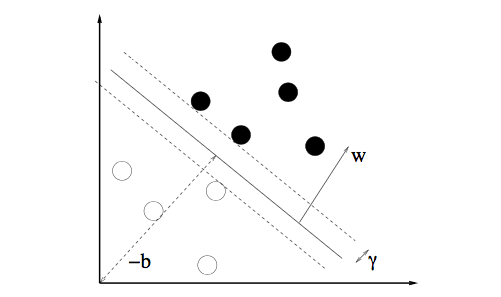
\includegraphics[width=1\linewidth]{adit_pics/svm-hyperplane}
	\caption{Hyperplane SVM pada \citep{fradkin2006support}}
	\label{fig:svm}
\end{figure}

Konsep dari cara SVM bekerja adalah dengan menemukan sebuah \textit{hyperplane} dengan \textit{margin} (jarak dari \textit{hyperplane} dengan titik kelas terdekat) yang terbesar. Pemilihan \textit{margin} dengan nilai terbesar ini ditujukan agar \textit{classifier} lebih optimal dalam memisahkan objek dengan kelas yang berbeda.

\section{Word Embedding Language Model}
Terdapat beberapa cara untuk merepresentasikan sebuah kata sebagai \textit{input model}. Salah satu cara yang sederhana adalah dengan merepresentasikan kata sebagai \textit{one hot vector}. Pada model ini, setiap kata di dalam sebuah korpus diberikan nomor indeks untuk membangun vektor yang mewakili keberadaan kata tersebut. Jika terdapat sebuah kata yang muncul pada konteks yang ingin direpresentasikan, indeks vektor yang sama dengan indeks kata tersebut akan bernilai 1. Bila terdapat sebuah korpus dengan jumlah kata unik berjumlah 4 dengan kata-kata "Ani", "marah", "kemarin", dan "malam" (sebuah vektor dengan pangjang empat). Representasi \textit{one hot vector} untuk kalimat "Ani marah" dapat ditulis dengan vektor [1,1,0,0].

Representasi \textit{one hot vector} akan mempunyai panjang vektor yang besar jika korpus mempunyai jumlah kata unik yang besar. Terdapat bentuk representasi lain untuk membentuk vektor dari kata, salah satunya adalah dengan \textit{word embedding}. \textit{Word Embedding} menggunakan representasi bilangan \textit{real} pada vektor untuk merepresentasikan sebuah kata berdasarkan hasil \textit{training} dengan suatu korpus. Contoh representasi dari \textit{word embedding} pada suatu kata "makan" adalah vektor [0.6, -0.3, ..., 0.5] (misalnya). Vektor dari hasil \textit{word embedding} mempunyai karakteristik dimana jarak antara dua buah vektor dari kata yang mirip secara semantik bernilai kecil(dekat). Bila misalkan pada data \textit{training} untuk \textit{word embedding} terdapat banyak kalimat-kalimat berbentuk "... makan Y ..." dimana Y adalah sebuah objek berupa makanan. Maka kata-kata yang mewakili Y seperti misalnya "burger", "apel", "steak", dan lain-lain, akan memiliki vektor yang mirip dan secara implisit dapat saling menggantikan untuk menempati posisi Y tersebut. Berdasarkan keterdekatan vektor tersebut, \textit{word embedding} mampu untuk menangkap semantik dari kata-kata yang ada pada korpus.

Salah satu model \textit{word embedding} yang dapat digunakan adalah Word2Vec \citep{mikolov2013distributed}. Terdapat dua buah arsitektur Word2Vec tersebut, yaitu skip-Gram dan \textit{Continous bag-of-words} (CBOW). Arsitektur pada CBOW memiliki pendekatan untuk memprediksi setiap kata berdasarkan kata-kata disekelilingnya. Lain halnya dengan arsitektur tersebut, Skip-Gram akan memprediksi kata-kata di sekeliling berdasarkan kata yang diberikan. Gambaran dari skip-gram dan CBOW dapat dilihat pada gambar berikut:

\begin{figure}
	\centering
	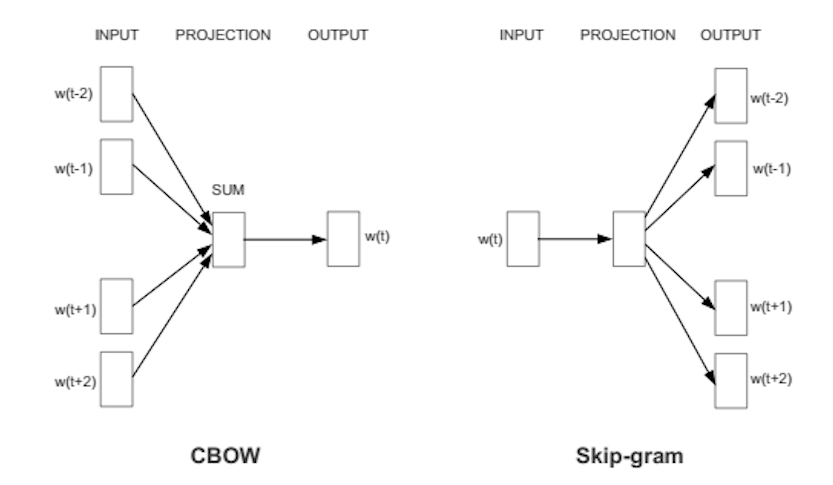
\includegraphics[width=1\linewidth]{adit_pics/word2vec_diagrams.png}
	\caption{Word2Vec}
	\label{fig:Word2Vec}
\end{figure}